\documentclass{article}
\usepackage{graphicx}
\usepackage{listings}
\usepackage{enumitem}
\usepackage{hyperref}
\usepackage[section]{placeins}
\usepackage[total={8in, 10in}]{geometry}
\lstset{
  breaklines=true,
  frame=single,
  gobble=12,
  tabsize=4,
  language=bash,
  basicstyle=\small\ttfamily,
  columns=fullflexible,
  showstringspaces=false
}

\author{Iresh Dissanayaka}

\title{Enabling HTTPS Communication for IBM AppConnect Integrations}

\begin{document}
    \maketitle

    \section{Introduction}
    This document is intended to be a guide to secure http communication in IBM App AppConnect Enterprise by enabling TLS (Transport Layer Security).
    
    \bigbreak
    
    The document only covers enabling https for the http applications hosted in an existing integration node setup.

    \section{Quick TLS/SSL Guide}
    If you need an introduction, please follow this link: \url{https://youtu.be/i-rtxrEz_E8}

    \begin{itemize}
        \item TLS can be considered the newer version of SSL. Terms are used interchangeably
        \item TLS utilizes PKI (Public Key Infrastructure) to do what it does
        \item TLS is what makes HTTP into HTTPS. When TLS is enabled, so is HTTPS
    \end{itemize}

    In our case, the intergration node (`server') is authenticated to the clients. In other words clients verify the identity of the intergration node. So, the client knows that it is communicating with the authentic server (the integration node) and can continue the communication securely.  This is same as how a HTTPS enabled website works. Website authenticates its identity to the users and encrypt further communication.
    
    \section{Configuring TLS/SSL for an integration node}
    \label{section_config_node}
    Configuring TLS/SSL is just providing the certificates and the private key (along with some parameters) to the intergration node using a standardized way. This guide assumes that you already have an integration node running.

    \subsection{Prerequisites}
    \begin{itemize}
        \item An integration node running
        \item Certificate for the integration node and the corresponding private key
        \item Certificate of the CA by which integration node certificate has been signed
    \end{itemize}

    \subsection{Procedure outline}
    \begin{enumerate}
        \item Gather the certificate files and the private key
        \item Ensure all the files are in PEM format and verify them
        \item Create a keystore and import the certificates
        \item Provide the keystore to the integration node
    \end{enumerate}

    \subsection{Procedure}
    This section describes outlined procudure in detail. The following set of variables are defined to improve the clarity of the guide.
    \begin{itemize}
        \item \lstinline{$NODE} : Name of the integration node, If it is \texttt{BRKR1}, Run,
        \begin{lstlisting}
            NODE=BRKR1
        \end{lstlisting}
        \item \lstinline{$CA_CERT} : Certificate file of CA
        \item \lstinline{$NODE_CERT} : Certificate file of the integration node
        \item \lstinline{$NODE_CERT_PRIV} : Private key of the certificate of the integration node
    \end{itemize}
    \subsubsection{Gather the certificate files and the private key}
    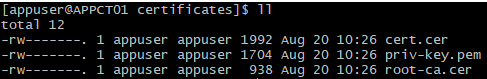
\includegraphics[width=\textwidth,height=\textheight,keepaspectratio]{cert-ls.png}
    \begin{itemize}
        \item \texttt{cert.cer} is the integration node's certificate. Run,
        \begin{lstlisting}
            NODE_CERT=cert.cer
        \end{lstlisting}
        \item \texttt{priv-key.pem} is the corresponding private key. Run,
        \begin{lstlisting}
            NODE_CERT_PRIV=priv-key.pem
        \end{lstlisting}
        \item \texttt{root-ca.cer} is the CA's certificate. Run,
        \begin{lstlisting}
            CA_CERT=root-ca.cer
        \end{lstlisting}
    \end{itemize}
    \textbf{These file names are as examples only. Please substitute the correct file names according to your setup.}

    \subsubsection{Ensure all the files are in PEM format and verify them}
    Please note that the file extension doesn't have to be \texttt{.pem} but can be. You need to check what's inside a file in order to verify whether it is PEM encoded. A certificate is most probably in PEM format or DER binary format.

    \begin{enumerate}[itemsep=3ex]
        \item Ensure node certificate is in PEM


        The certificate file might be encoded in PEM (regardless of the file extension) or DER binary format. To check whether it is in PEM, run,
        \begin{lstlisting}
            openssl x509 -in $NODE_CERT -subject -noout
        \end{lstlisting}
        If it says something similar to following, it is in PEM.
        \begin{lstlisting}
            subject= /C=LK/ST=WESTERN/L=COLOMBO 3/O=DFCC BANK PLC/OU=IT/CN=esbprod.dfcc.net
        \end{lstlisting}
        else if it says something similar to following, it is probably in DER
        \begin{lstlisting}
            unable to load certificate
            139778153113488:error:0906D06C:PEM routines:PEM_read_bio:no start line:pem_lib.c:707
        \end{lstlisting}
        then run the following to check whether it is DER,
        \begin{lstlisting}
            openssl x509 -inform der -in $NODE_CERT -subject -noout
        \end{lstlisting}
        If it says something similar to following, it is in DER.
        \begin{lstlisting}
            subject= /C=LK/ST=WESTERN/L=COLOMBO 3/O=DFCC BANK PLC/OU=IT/CN=esbprod.dfcc.net
        \end{lstlisting}
        if that results an error as well, something might be wrong. Check your certificate file.

        
        If your certificate file was in DER, convert that to PEM and replace the original file. Run,
        \begin{lstlisting}
            openssl x509 -inform der -in $NODE_CERT -outform pem -out $NODE_CERT.pem
            mv $NODE_CERT.pem $NODE_CERT
        \end{lstlisting}

        \item Ensure CA certificate is in PEM

        It is pretty much the same for CA certificate as well.


        The certificate file might be encoded in PEM (regardless of the file extension) or DER binary format. To check whether it is in PEM, run,
        \begin{lstlisting}
            openssl x509 -in $CA_CERT -subject -noout
        \end{lstlisting}
        If it says something similar to following, it is in PEM.
        \begin{lstlisting}
            subject= /DC=net/DC=dfcc/CN=dfcc-ROOTAD-CA-1
        \end{lstlisting}
        else if it says something similar to following, it is probably in DER
        \begin{lstlisting}
            unable to load certificate
            139778153113488:error:0906D06C:PEM routines:PEM_read_bio:no start line:pem_lib.c:707
        \end{lstlisting}
        then run the following to check whether it is DER,
        \begin{lstlisting}
            openssl x509 -inform der -in $CA_CERT -subject -noout
        \end{lstlisting}
        If it says something similar to following, it is in DER.
        \begin{lstlisting}
            subject= /DC=net/DC=dfcc/CN=dfcc-ROOTAD-CA-1
        \end{lstlisting}
        if that results an error as well, something might be wrong. Check your certificate file.


        If your certificate file was in DER, convert that to PEM and replace the original file. Run,
        \begin{lstlisting}
            openssl x509 -inform der -in $CA_CERT -outform pem -out $CA_CERT.pem
            mv $CA_CERT.pem $CA_CERT
        \end{lstlisting}

        \item Verify the private key file. Run,
        \begin{lstlisting}
            openssl rsa -in $NODE_CERT_PRIV -check -noout
        \end{lstlisting}
        Example output:
        \begin{lstlisting}
            RSA key ok
        \end{lstlisting}

        \item Verify that the certificate and the private key match. Run,
        \begin{lstlisting}
            test "$(openssl x509 -in $NODE_CERT -modulus -noout)" = "$(openssl rsa -in $NODE_CERT_PRIV -modulus -noout)" && echo OK
        \end{lstlisting}
        Example output:
        \begin{lstlisting}
            OK
        \end{lstlisting}

    \end{enumerate}

    \subsubsection{Create a keystore and import the certificates}
    Idea here is to bundle all three files into a single file called a `keystore'.

    \begin{enumerate}[itemsep=4ex]
        \item Create a \texttt{.pfx} file to contain the integration node's certificate and the corresponding private key and the CA certificate.

        Now what we have is the following set of files,
        \begin{itemize}
            \item Certificate file of the integration node in PEM format (\lstinline{$NODE_CERT})
            \item CA certificate file in PEM format (\lstinline{$CA_CERT})
            \item Private key file of the certificate of the integration node in PEM format (\lstinline{$NODE_CERT_PRIV})
        \end{itemize}

        Run the following commmand to create the \texttt{bundle.pfx} file.
        \begin{lstlisting}
            openssl pkcs12 -export -inkey $NODE_CERT_PRIV -in $NODE_CERT -name $NODE-cert -caname root-ca-cert -certfile $CA_CERT -out ${NODE}-bundle.pfx
        \end{lstlisting}
        You'll be prompted to enter an export password. Please remember the password you enter.

        \item Create the keystore and import the certificates and the private key

        We are going to use IBM's Global Security Kit (GSKit) to create the keystore. Please install it if not installed already. If there is a MQ installation, it contains the GSKit as well. We are going to use the GSKit installation that comes with the MQ installation for this guide.
        \begin{enumerate}
            \item Prepare the environment for running necessary commands. Run, (please use the correct paths according to your environment)
            \begin{itemize}
                \item \lstinline{<app_connect_installation_root>}, example: \lstinline{/opt/IBM/ace/ace-11.0.0.11}
                \item \lstinline{<mq_installation_root>}, example: \lstinline{/opt/mqm}
            \end{itemize}
            \begin{lstlisting}
                source <app_connect_installation_root>/server/bin/mqsiprofile -s
                PATH=$PATH:<mq_installation_root>/gskit8/bin
                LD_LIBRARY_PATH=$LD_LIBRARY_PATH:<mq_installation_root>/gskit8/lib64
            \end{lstlisting}
            \item Create the keystore which is just a file. Keystore type will be P12 and we'll name the file \texttt{node\_keystore.p12}. Run, (you need to choose a password for the \lstinline{<keystore_password>} \label{keystore_password} and it'll be needed for subsequent steps)
            \begin{lstlisting}
                gsk8capicmd_64 -keydb -create -db $NODE_keystore.p12 -type p12 -pw <keystore_password>
            \end{lstlisting}
            \item Import the integration node's certificate and the private key to the keystore (Replace \lstinline{$EXPASS} with the export password you entered when creating the bundle.pfx file). Run,
            \begin{lstlisting}
                gsk8capicmd_64 -cert -import -db bundle.pfx -type p12 -pw $EXPASS  -label node-cert -target ${NODE}_keystore.p12 -target_pw <kekystore_password> -target_type p12
            \end{lstlisting}
            \item Import the CA certificate to the keystore. Run,
            \begin{lstlisting}
                gsk8capicmd_64 -cert -import -db bundle.pfx -type p12 -pw $EXPASS -label root-ca-cert -target ${NODE}_keystore.p12 -target_pw <keystore_password> -target_type p12
            \end{lstlisting}
        \end{enumerate}

    \end{enumerate}
    \subsubsection{Provide the keystore to the integration node}
    Once you have the keystore ready, you need to configure integration node so that it can access the keystore.
    Suppose that the keystore is stored in the following directory,
    \begin{lstlisting}[gobble=8]
        /etc/ace_tls/
    \end{lstlisting}

    Integration node's broker registry is configured so that the parameters will be applied to all the server listeners and the node listener.
    \begin{enumerate}
        \item Set the keystore path. Run,
        \begin{lstlisting}
            mqsichangeproperties $NODE -o BrokerRegistry -n brokerKeystoreFile -v /etc/ace_tls/${NODE}_keystore.p12
        \end{lstlisting}
        \item Set the keystore type which is P12. Run,
        \begin{lstlisting}
            mqsichangeproperties $NODE -o BrokerRegistry -n brokerKeystoreType -v P12
        \end{lstlisting}
        \item Set the \lstinline{<keystore_password>} you used when creating the keystore in \ref{keystore_password} in subsection 3.3.3. Run,
        \begin{lstlisting}
            mqsisetdbparms $NODE -n brokerKeystore::password -u ignore -p <keystore_password>
        \end{lstlisting}
        \item Restart the integration node. Run,
        \begin{lstlisting}
            mqsistop $NODE
            mqsistart $NODE
        \end{lstlisting}
    \end{enumerate}
    \subsubsection{Test HTTPS}
    \label{test_https}
    This section describes how you can test HTTPS connectivity using a sample application.

    \begin{enumerate}
        \item Obtain the \texttt{SimpleAppHTTPS.bar} file supplied along with the documentation
        \item Deploy the \texttt{SimpleAppHTTPS.bar} file to an integration server under the integration node. Run,
        \begin{lstlisting}
            mqsideploy $NODE -e <server_name> -a SimpleAppHTTPS.bar
        \end{lstlisting}
        \item Run a sample request and verify. Run,
        \begin{lstlisting}
             curl --cacert $CA_CERT -X POST https://localhost:7083/Echo -d HelloWorld && echo
        \end{lstlisting}
        Expected output:
        \begin{lstlisting}
            HelloWorld
        \end{lstlisting}
    \end{enumerate}
    If you got the expected output, you have configured HTTPS successfully.
    
    \section{Configuring the specific HA setup}
    Following figure illustrates the target setup.
    \begin{itemize}
        \item There are two integration nodes \texttt{BRDFC1} and \texttt{BRDFC2} spread across two VMs \texttt{APPCT01} and \texttt{APPCT02}
        \item Each integration node involves two instances, one active and one standby
        \item For a given integration node, both instances share a single broker registry. Therefore, parameters set targetting one of the instances applies to both
    \end{itemize}

    \begin{figure}[h]
        \centering
        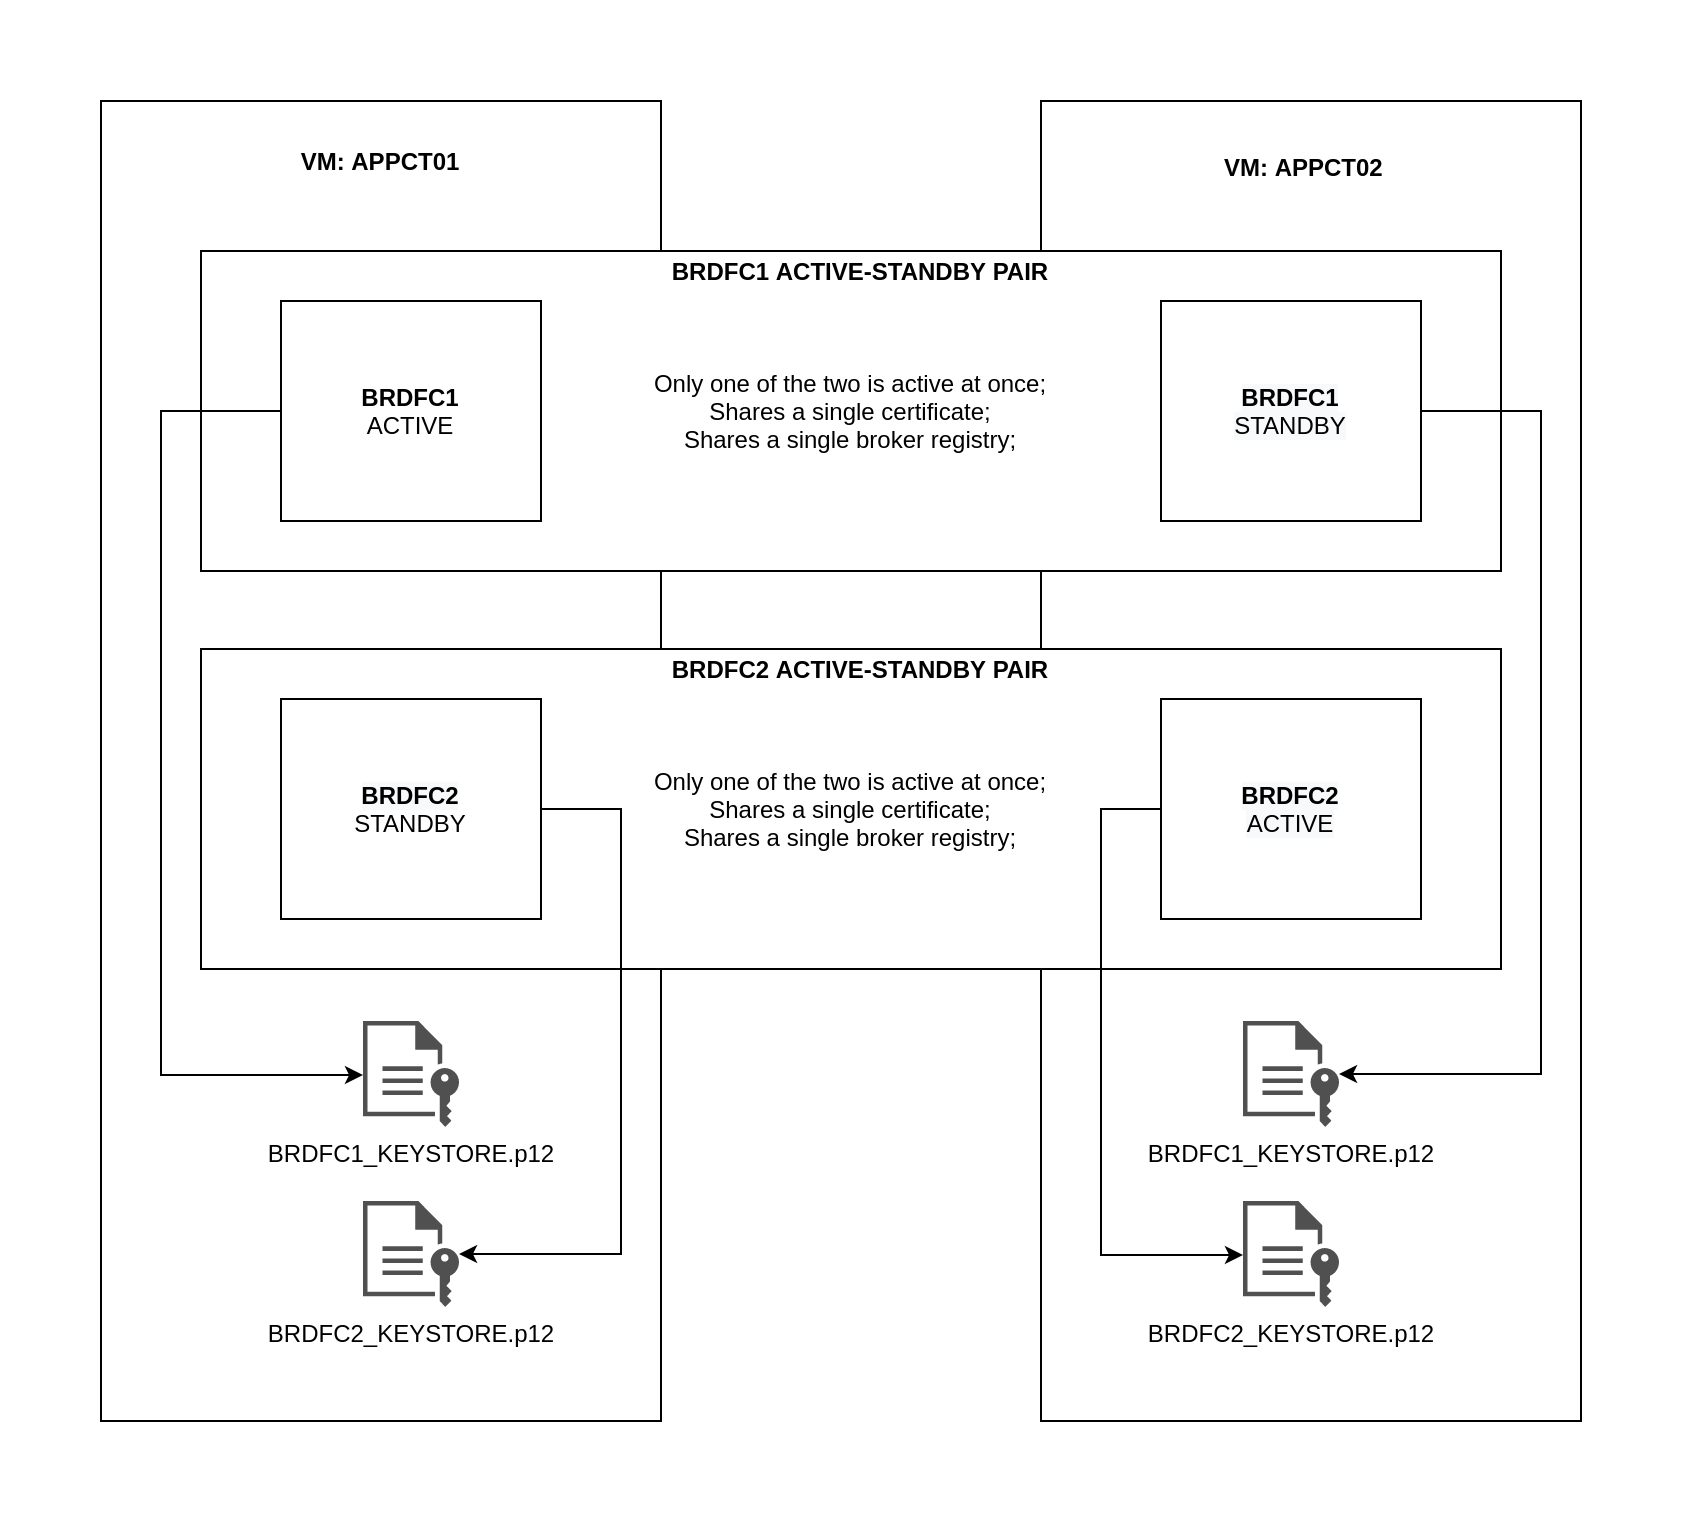
\includegraphics[width=\textwidth,height=\textheight,keepaspectratio]{ha-setup.png}
    \end{figure}
    \FloatBarrier

    \subsection{Procedure}
    There should be a certificate and a private key for each of the nodes. Therefore, following set of files should be available, (Please note that the file names might be different. Substitute them with the ones you have.)
    
    \begin{itemize}
        \item CA certificate \texttt{root-ca-cert.cer}
        \item \texttt{BRDFC1} certificate \texttt{brdfc1\_cert.cer}
        \item \texttt{BRDFC2} certificate \texttt{brdfc2\_cert.cer}
        \item \texttt{BRDFC1} certificate's private key \texttt{brdfc1\_priv.key}
        \item \texttt{BRDFC2} certificate's private key \texttt{brdfc2\_priv.key}
    \end{itemize}


    \subsubsection{Configure two nodes using the method described in section \ref{section_config_node}} 
    \begin{itemize}
        \item Cofigure the BRDFC1 node by logging in to the APPCT01 VM and following the instructions in section \ref{section_config_node}
        \item Cofigure the BRDFC2 node by logging in to the APPCT02 VM and following the instructions in section \ref{section_config_node}
    \end{itemize}

    \subsubsection{Make both configured keystores available on same paths on both VMs} 
    \begin{itemize}
        \item Copy over the keystore on APPCT01 VM to the exactly same path on APPCT02 VM and vice versa

        For example,
        
        if \lstinline{BRDFC1_keystore.p12} is on the VM \texttt{APPCT01} at path \lstinline{/etc/ace_tls/BRDFC1_keystore.p12}, copy it to the same path on the VM \texttt{APPCT02}. Run on VM \texttt{APPCT01},
        \begin{lstlisting}
            scp /etc/ace_tls/BRDFC1_keystore.p12 <appct02_username>@APPCT02:/etc/ace_tls/
        \end{lstlisting}
        
        if \lstinline{BRDFC2_keystore.p12} is on the VM \texttt{APPCT02} at path \lstinline{/etc/ace_tls/BRDFC2_keystore.p12}, copy it to the same path on the VM \texttt{APPCT01}. Run on VM \texttt{APPCT02},
        \begin{lstlisting}
            scp /etc/ace_tls/BRDFC2_keystore.p12 <appct01_username>@APPCT01:/etc/ace_tls/
        \end{lstlisting}
    \end{itemize}

    \subsubsection{Test connectivity}
    \begin{itemize}
        \item Follow section \ref{test_https} to test HTTPS connectivity for each integration node
        \item Simulate failover scenario and repeat the same. (You might need to adjust IP/hostname and the ports accordingly)
    \end{itemize}

\end{document}